\documentclass[12pt, leqno]{article} %% use to set typesize
\input{common}

\usepackage{fontspec}
\usepackage{polyglossia}
\setmonofont{DejaVu Sans Mono}[Scale=MatchLowercase]
\usepackage[outputdir=pdf]{minted}

\providecommand{\tightlist}{%
  \setlength{\itemsep}{0pt}\setlength{\parskip}{0pt}}
\begin{document}



\hdr{2023-04-19}

\section{Levenberg-Marquardt}

Recall from our discussion of nonlinear least squares the
Levenberg-Marquardt iteration where we solve a \emph{regularized} least
squares problem to compute the step; that is,
\[p_k = \operatorname{argmin}_p
    \frac{1}{2} \|f(x_k) + f'(x_k) p\|^2 +
    \frac{\mu}{2} \|Dp\|^2.\] The scaling matrix \(D\) may be an
identity matrix (per Levenberg), or we may choose
\(D^2 = \operatorname{diag}(f'(x_k)^T f'(x_k))\) (as suggested by
Marquardt).

For \(\lambda = 0\), the Levenberg-Marquardt step is the same as a
Gauss-Newton step. As \(\lambda\) becomes large, though, we have the
(scaled) gradient step
\[p_k = -\frac{1}{\mu} D^{-2} f'(x_k)^T f(x_k) + O(\mu^{-2}).\] Unlike
Gauss-Newton with line search, changing the parameter \(\mu\) affects
not only the distance we move, but also the direction.

In order to get both ensure global convergence (under sufficient
hypotheses on \(f\), as usual) and to ensure that convergence is not too
slow, a variety of methods have been proposed that adjust \(\lambda\)
dynamically. To judge whether \(\mu\) has been chosen too aggressively
or conservatively, we monitor the \emph{gain ratio}, or the ratio of
actual reduction in the objective to the reduction predicted by the
(Gauss-Newton) model: \[\rho =
  \frac{\|f(x_k)\|^2-\|f(x_k+p_k)\|^2}
       {\|f(x_k)\|^2 - \|f(x_k)+f'(x_k)p_k\|^2}.\] If the step decreases
the function value enough (\(\rho\) is sufficiently positive), then we
accept the step; otherwise, we reject it. For the next step (or the next
attempt), we may increase or decrease the damping parameter \(\mu\)
depending on whether \(\rho\) is close to one or far from one.

\begin{minted}{julia}
function levenberg_marquardt(x0, f, J; nsteps=100, rtol=1e-8, τ=1e-3,
                             monitor=(x, rnorm, μ))
    
    # Evaluate everything at the initial point
    x = copy(x0)
    Jx = J(x)
    fx = f(x)
    Hx = Jx'*Jx

    μ = τ * maximum(diag(Hx))  # Default damping parameter
    ν = 2.0                    # Step re-scaling parameter (default value)
    
    for k = 1:nsteps
        
        # Check for convergence
        g = Jx'*fx
        rnorm = norm(Jx'*fx)
        monitor(x, rnorm, μ)
        if rnorm < rtol
            return x
        end
        
        # Compute a proposed step and re-evaluate residual vector
        p = (Hx + μ*I)\(-g)
        xnew = x + p
        fxnew = f(xnew)
        
        # Compute the gain ratio
        ρ = (norm(fx)^2 - norm(fxnew)^2) / (norm(fx)^2 - norm(fx+Jx*p)^2)
        
        if ρ > 0  # Success!
            
            # Accept new point
            x = xnew
            fx = fxnew
            Jx = J(x)
            Hx = Jx'*Jx
            
            # Reset re-scaling parameter, update damping
            μ *= max(1.0/3.0, 1.0-2.0*(ρ-1.0)^3)
            ν = 2.0
        
        else
                
            # Rescale damping
            μ *= ν
            ν *= 2.0

        end
    end
    error("Did not converge in $nsteps iterations")
end
\end{minted}

\section{Consider constraints}

There is another way to think of the Levenberg-Marquardt step. Consider
the minimization problem
\[p_k = \operatorname{argmin}_p \frac{1}{2} \|f(x) + f'(x)p \|^2 \mbox{ s.t. }
  \|Dp\| \leq \Delta.\]

There are two possible cases in this problem:

\begin{enumerate}
\def\labelenumi{\arabic{enumi}.}
\tightlist
\item
  \(\|f'(x_k)^\dagger f(x)\| < \Delta\), and the solution is the
  Gauss-Newton step
\item
  Otherwise the Gauss-Newton step is too big, and we have to enforce the
  constraint \(\|Dp\| = \Delta\). For convenience, we rewrite this
  constraint as \((\|Dp\|^2-\Delta^2)/2 = 0\).
\end{enumerate}

We define the Langrangian for the optimization problem to be
\[L(p,\lambda) =
    \frac{1}{2} \|f(x_k)+f'(x_k) p\|^2 +
    \frac{\lambda}{2} \left( \|Dp\|^2-\Delta^2 \right).\] The solution
to the constrained optimization problem satisfies the critical point
equation \(\partial L/\partial p = 0\) and
\(\partial L/\partial \lambda = 0\). The equation
\(\partial L/\partial p = 0\) is the same as the Tikhonov-regularized
least squares problem with regularization parameter \(\lambda\). Whether
\(\lambda\) is treated as a regularization parameter or a multiplier
that enforces a constraint is thus simply a matter of perspective.
Hence, we can consider the Levenberg-Marquardt method as minimizing the
model \(\|f(x_k) + f(x_k) p\|\) subject to the constraint
\(\|Dp\| \leq \Delta\), where a larger or smaller value of \(\lambda\)
corresponds to a smaller or larger value of \(\Delta\). We think of the
region \(\|Dp\| \leq \Delta\) as the region where the Gauss-Newton model
provides good guidance for optimization; that is, it is a region where
we trust the model.

\section{Trust regions}

A \emph{trust region} method for mininizing \(\phi\) involves a
\emph{model} \(\mu(p)\) that is supposed to approximate the decrease
\(\phi(x_k+p)-\phi(x_k)\) associated with taking a step \(p\); and a
\emph{trust region}, often chosen to be a sphere \(\|p\| \leq \Delta\),
where we believe the model to provide reasonable predictions.

The simplest model \(\mu(p)\) is linear, but the more interesting (and
common) case involves a quadratic model
\[\mu(p) = g^T p + \frac{1}{2} p^T H p.\] Minimizing a quadratic
\(\mu(p)\) subject to the constraint \(\|\mu(p)\| \leq \Delta\) is
\emph{not} easy. We turn to this \emph{trust region subproblem} next.

Compared to a line search strategy, trust region methods have the
advantage that we adapt not just the step length but also the direction
of the search. Consequently, trust region methods often exhibit more
robust convergence, though both line search and trust region approaches
exhibit good global convergence properties, and both approaches lead to
eventual superlinear convergence when paired with a Newton model (i.e.~a
quadratic approximation centered at \(x_k\)) or a quasi-Newton method
such as BFGS.

\subsection{The trust region subproblem}

The problem
\[\mbox{minimize } g^T p + \frac{1}{2} p^T H p \mbox{ s.t. } \|p\| \leq \Delta\]
is the \emph{trust region subproblem}. Sometimes people use the more
general constraint \[p^T M p \leq \Delta^2\] for some positive definite
\(M\), but we will stick to the usual 2-norm. There are two possible
solutions:

\begin{enumerate}
\def\labelenumi{\arabic{enumi}.}
\tightlist
\item
  If \(H\) is positive definite and \(\|H^{-1} g\| \leq \Delta\), then
  the solution is \(p = -H^{-1} g\). This is the \emph{interior} case.
\item
  If \(H\) is not positive definite or \(\|H^{-1} g\| > \Delta\), then
  the solution iis \(p = -(H+\lambda I)^{-1} g\) for some
  \(\lambda > 0\) such that \(\|p\| = \Delta\). At the appropriate
  \(\lambda\), we have \(H+\lambda I\) is positive semi-definite. This
  is the \emph{boundary case}
\end{enumerate}

Most of the effort is spent on the boundary case, which itself has two
subcases:

\begin{enumerate}
\def\labelenumi{\arabic{enumi}.}
\tightlist
\item
  If \(H + \lambda I\) is positive definite, then there is a unique
  solution to the trust region subproblem.
\item
  If \(H + \lambda I\) is singular, then there are multiple solutions to
  the trust region subproblem, and we seen the problem with minimum
  norm.
\end{enumerate}

The case when \(H + \lambda I\) is singular (i.e.~\(-\lambda\) is an
eigenvalue of \(H\)) is consistently known as the \emph{hard case} in
the literature.

\subsection{Exact solves}

The standard solver for the trust-region subproblem is due to
\href{https://doi.org/10.1137/0904038}{Moré and Sorensen}, and involves
a safeguarded Newton iteration for finding the relevant \(\lambda\),
with careful treatment of the hard case. A number of authors have also
adapted this approach to the large sparse case. However, I am
particularly fond of a method proposed by
\href{https://doi.org/10.1007/978-3-642-75536-1_57}{Gander, Golub, and
Von Matt} that recasts the trust-region subproblem in terms of an
eigenvalue problem. That paper concluded that the eigenvalue formulation
was numerically inferior to the Moré-Sorensen approach, but a 2017 paper
of \href{https://doi.org/10.1137/16M1058200}{Adachi, Iwata, Nakatsukasa,
and Takeda} concluded that this was in part because the eigensolvers
available in 1989 were not as good as the solvers currently available.
The Adachi et al paper provides a nice discussion of the formulation,
including the hard case, which results in a mercifully brief code (which
you are nonetheless not required to digest). One of the nice things
about this formulation is that it adapts naturally to large-scale
problems where \(H\) is sparse or data sparse, though we will only worry
about the dense case in our code.

\begin{minted}{julia}
function solve_tr(g, H, Δ)
    n = length(g)

    # Check interior case
    try
        F = cholesky(H)
        p = -(F\g)
        if norm(p) <= Δ
            return p, false
        end
    catch e
        # Hit this case if Cholesky errors (not pos def)
    end    

    # Compute the relevant eigensolve
    w = g/Δ
    M = [H    -I ;
         -w*w' H ]
    λs, V = eigen(M)
    
    # The right most eigenvalue (always sorted to the end in Julia) is real,
    # and corresponds to the desired λ
    λ = -real(λs[1])
    v = real(V[:,1])
    y2 = v[1:n]
    y1 = v[n+1:end]
    
    # Check if we are in the hard case (to some tolerance)
    gap = real(λs[2])-real(λs[1])
    if norm(y1) <= 1e-8/sqrt(gap)
        # Hard case -- we punt a little and assume only one null vector
        #  Compute min-norm solution plus a multiple of the null vector.
        v = y2/norm(y2)
        q = -(H+norm(H)/n^2*v*v')\g
        return q + v*sqrt(Δ^2-q'*q), true
    else
        # Standard case -- extract solution from eigenvector
        return -sign(g'*y2) * Δ * y1/norm(y1), true
    end
end
\end{minted}

\begin{figure}
\begin{center}
  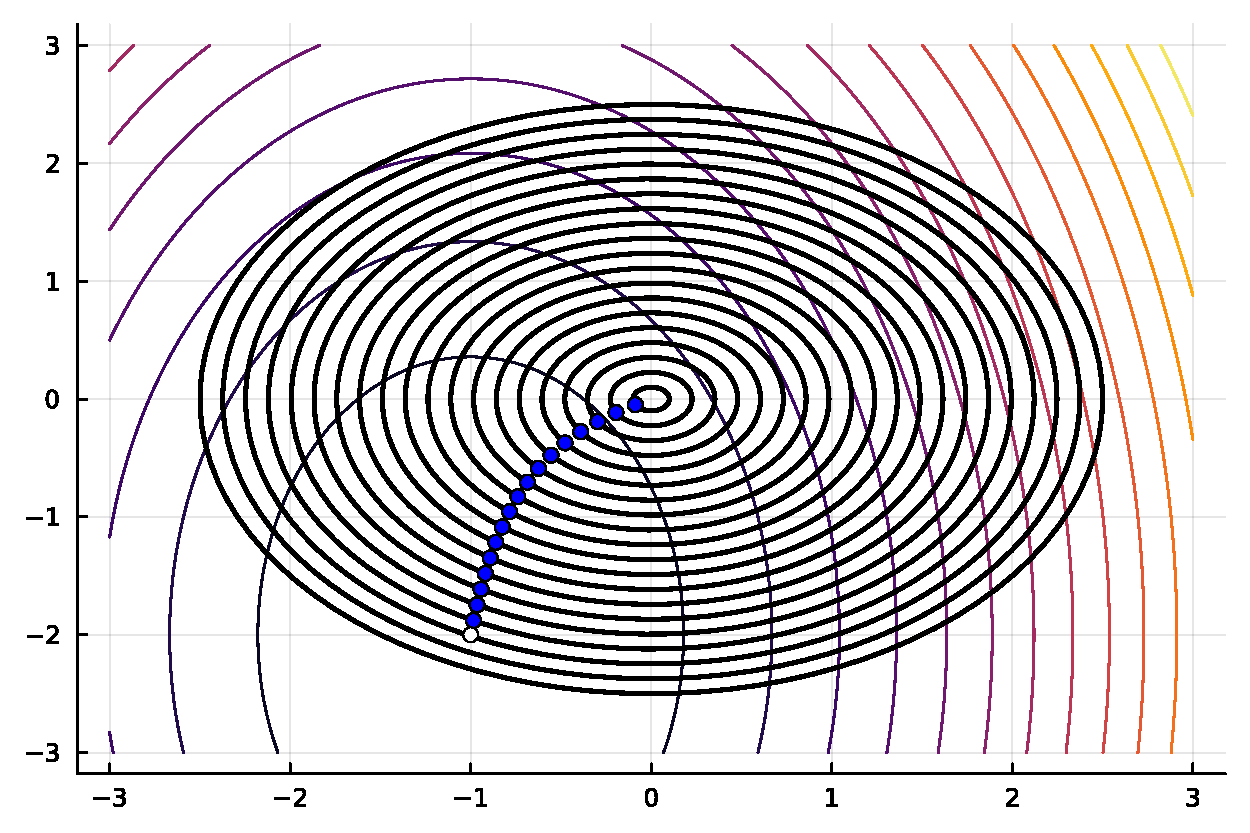
\includegraphics[width=0.8\textwidth]{fig/2023-04-19-demo-tr1.pdf}
\end{center}
\caption{Plot of trust region subproblem solve for varying $\Delta$.}
\label{fig:demo-tr1}
\end{figure}

A useful picture is a plot of the step for various $\Delta$ values for
a sample quadratic model (Figure~\ref{fig:demo-tr1}).

\subsection{Inexact solves}

One of the main difficulties with the trust region approach is solving a
constrained quadratic optimization as a subproblem. As with line search,
the thinking goes, the cost of doing an exact search is probably not
worthwhile --- we would rather get a good-enough approximate solution
and move on.

A popular inexact search approach is the \emph{dog leg} method. The idea
of the dog leg method is to approximate the shape of the curve

\[p(\Delta) = \operatorname{argmin}_p \mu(p) \mbox{ s.t. } \|p\| \leq \Delta\]

based on the observation that

\begin{itemize}
\tightlist
\item
  \(p(0) = 0\).
\item
  \(p'(0) \propto -\nabla \phi(x_k)\).
\item
  For large \(\Delta\), \(p(\Delta) = p_{\infty}\) is the unconstrained
  minimizer of \(\mu\).
\end{itemize}

We thus approximate the \(\rho(\Delta)\) curve by a piecewise linear
curve with

\begin{itemize}
\tightlist
\item
  A line segment from \(0\) to \(-\alpha \nabla \phi(x_k)\) where
  \(\mu(-\alpha \nabla \phi(x_k))\) is mimimized.
\item
  Another line segment from \(-\alpha \nabla \phi(x_k)\) to
  \(p_{\infty}\).
\end{itemize}

\begin{minted}{julia}
function dogleg_tr(g, H, Δ)
    n = length(g)

    # Positive definite case (Cholesky succeeds)
    try
        F = cholesky(H)
        p∞ = -(F\g)
        
        # Check for interior case
        if norm(p∞) <= Δ
            return p∞, false
        end
        
        # Compute a Cauchy step (first part of the dog leg)
        τ = (g'*g)/(g'*H*g)
        pc = -τ*g
        if norm(pc) >= Δ
            return (Δ/norm(pc)) * pc, true
        end
        
        # If the Cauchy step is interior, do the dog leg:
        #   p = pc + η*(p∞-pc) s.t. norm(p) = Δ
        # This corresponds to solving the quadratic
        #   pc'*pc + 2*η*pc'*(p∞-pc) + η^2*(p∞-pc)'*(p∞-pc) = Δ^2
        #
        a = (p∞-pc)'*(p∞-pc)
        b = pc'*(p∞-pc)
        c = pc'*pc - Δ^2
        η = (-b + sqrt(b^2 - a*c))/a
        return pc + η*(p∞-pc), true

    catch e
        # Hit this case if Cholesky errors (not pos def)
    end    

    # Compute a Cauchy step
    τ = (g'*g)/(g'*H*g)
    pc = -τ*g
    if τ < 0.0 || norm(pc) >= Δ
        return (Δ/norm(pc)) * pc, true
    end
    return -(Δ/norm(g)) * g, true

end
\end{minted}

\begin{figure}
\begin{center}
  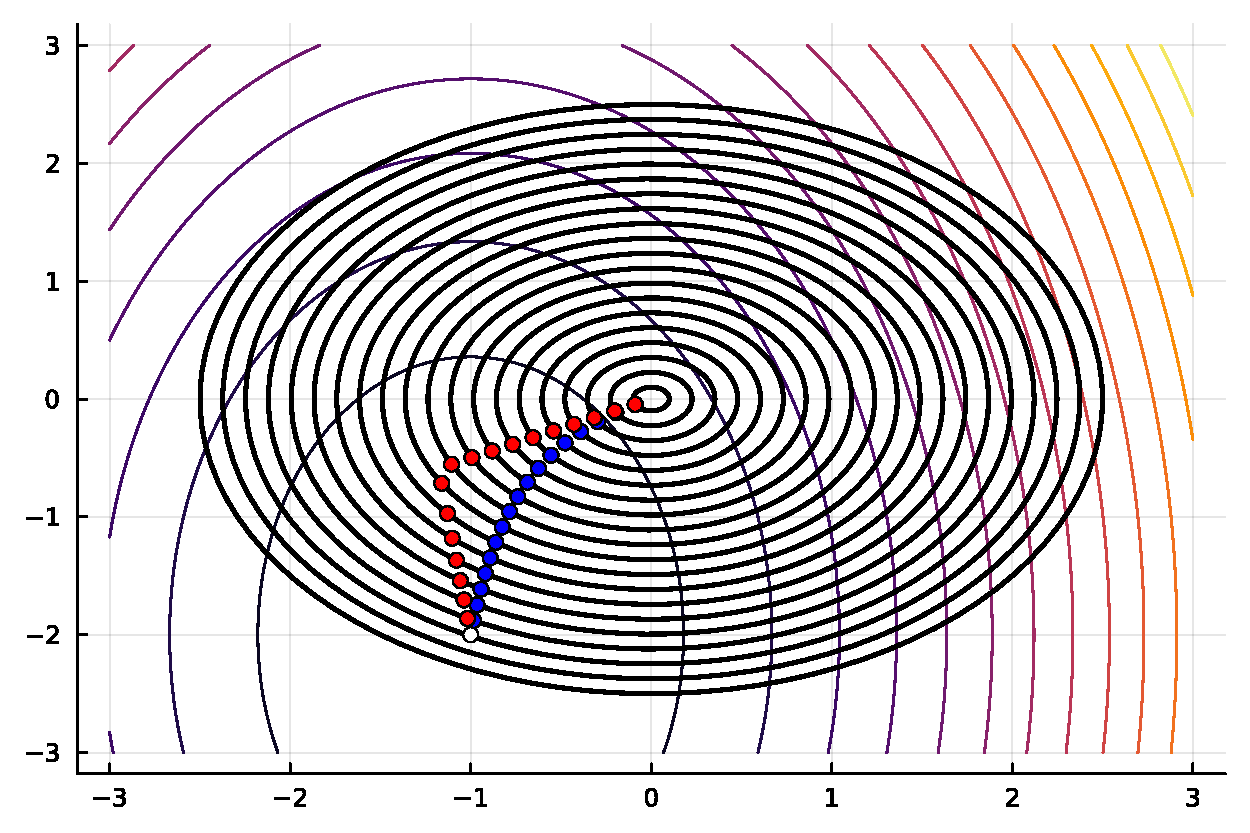
\includegraphics[width=0.8\textwidth]{fig/2023-04-19-demo-dogleg.pdf}
\end{center}
\caption{Plot of trust region subproblem dogleg approximation for 
  varying $\Delta$.}
\label{fig:demo-dogleg}
\end{figure}

A plot illustrates what happens with the dogleg path as a function of
$\Delta$, compared to the true trust region solution path: the dogleg
is a piecewise linear approximation to the true path
(Figure~\ref{fig:demo-dogleg}).

A related approach is \emph{two-dimensional subspace minimization},
which involves a constrained miminization over the two-dimensional
subspace spanned by \(-\nabla \phi(x_k)\) and \(p_{\infty}\).

The \emph{Steighaug} method combines the trust region approach with a
(linear) conjugate gradient solve on the quadratic model problem. The
idea is to trace out a polygonal path (as in the dog leg method)
connecting the CG iterates, until that path intersects the trust region
boundary. If the (approximate) Hessian used by the model is indefinite,
CG runs until it discovers the indefiniteness, then plots a path toward
where the model descends to \(-\infty\). There are more recent variants
which combine Newton, trust regions, and Krylov subspaces in various
clever ways; other than mentioning that they exist, though, we leave
this topic for the interested student to pursue in her copious free
time.

\subsection{Adapting the trust region}

At each step of the method, we (approximately) minimize the model within
the trust region to get a proposed step \(p\), then check the gain ratio
associated with taking that step:
\[\rho_k = \frac{\phi(x_k)-\phi(x_k+p_k)}{\mu(0)-\mu(p_k)}.\] Depending
on whether the gain ratio, we adjust \(\Delta\); a strategy proposed in
Nocedal and Wright is:

\begin{itemize}
\tightlist
\item
  If \(\rho_k < 1/4\), we were too aggressive; set
  \(\Delta_{k+1} = \Delta_k/4\).
\item
  If \(\rho_k > 3/4\) and \(\|p_k\| = \Delta_k\), we were too
  conservative; set \(\Delta_{k+1} = \min(2\Delta_k, \Delta_{\max})\).
\item
  Otherwise, leave \(\Delta_{k+1} = \Delta_k\).
\end{itemize}

We also use the gain ratio to decide whether to accept or reject the
step. For \(\rho_k > \eta\) for a fixed \(\eta \in [0,1/4)\), we accept
(\(x_{k+1} = x_k+p\)); otherwise we reject (\(x_{k+1} = x_k\)).

\begin{minted}{julia}
function tr_newton(x0, ϕ, ∇ϕ, Hϕ; nsteps=100, rtol=1e-6, Δmax=Inf,
                   monitor=(x, rnorm, Δ)->nothing)
    
    # Compute an intial step and try trusting it
    x = copy(x0)
    ϕx = ϕ(x)
    gx = ∇ϕ(x)
    Hx = Hϕ(x)
    p = -Hx\gx
    Δ = 1.2 * norm(p)^2
    hit_constraint = false
    
    for k = 1:nsteps

        # Compute gain ratio for new point and decide to accept or reject
        xnew = x + p
        ϕnew = ϕ(xnew)
        μdiff = -( gx'*p + (p'*Hx*p)/2 )
        ρ = (ϕx - ϕnew)/μdiff
        
        # Adjust radius
        if ρ < 0.25
            Δ /= 4.0
        elseif ρ > 0.75 && hit_constraint
            Δ = min(2*Δ, Δmax)
        end
        
        # Accept if enough gain (and check convergence)
        if ρ > 0.1
            x[:] = xnew
            ϕx = ϕnew
            gx = ∇ϕ(x)
            monitor(x, norm(gx), Δ)
            if norm(gx) < rtol
                return x
            end
            Hx = Hϕ(x)
        end

        # Otherwise, solve the trust region subproblem for new step
        p, hit_constraint = solve_tr(gx, Hx, Δ)

    end
    return x
end
\end{minted}

\subsection{An illustrative computation}

It is always useful to see how these things work on a problem we've
already looked at in another context. Let's consider as an example the
Rosenbrock banana function.

\begin{minted}{julia}
begin
    frosen(x) = 100*(x[2]-x[1]^2)^2 + (1-x[1])^2
    grosen(x) = [400*x[1]*(x[1]^2-x[2]) + 2*(x[1]-1);
    	         200*(x[2]-x[1]^2)]
    Hrosen(x) = [ 400*(3*x[1]^2-x[2])+2  -400*x[1] ;
    	          -400*x[1]               200   ]
end
\end{minted}

\begin{figure}
\begin{center}
  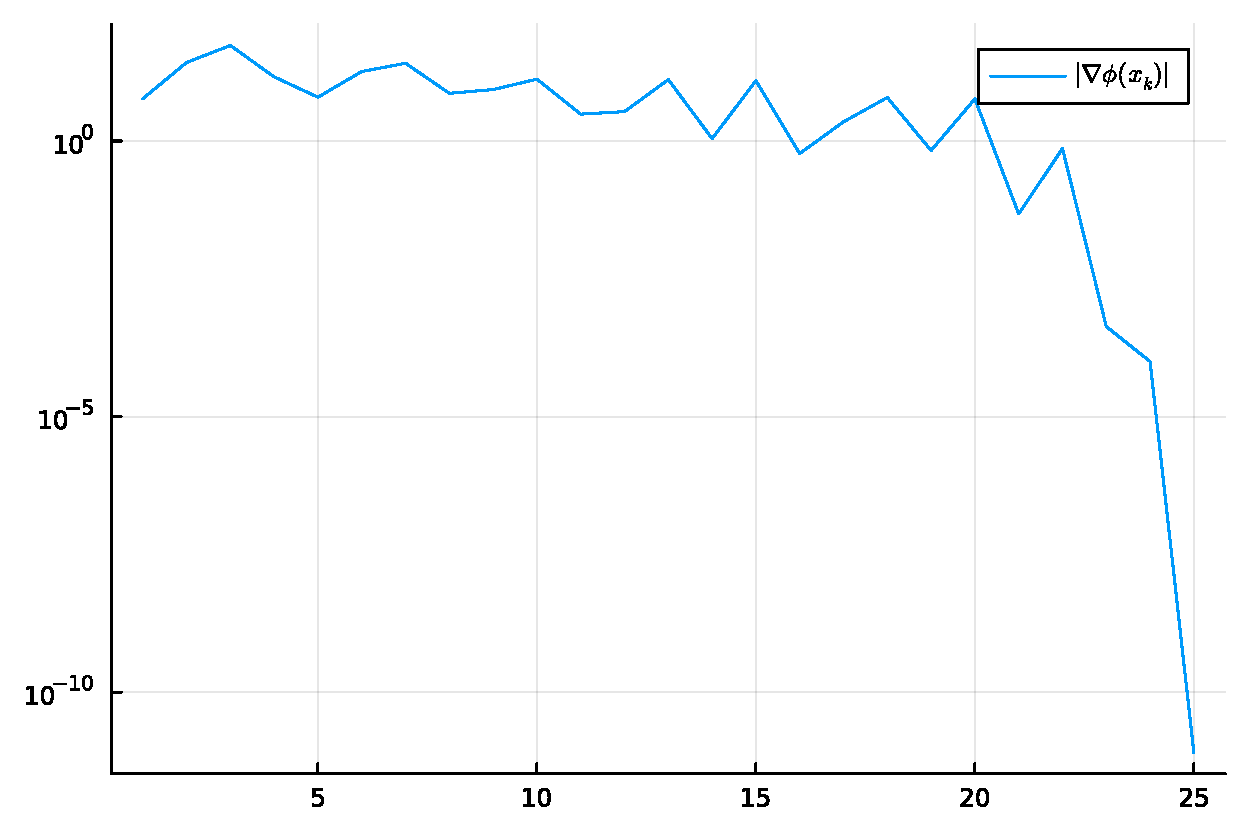
\includegraphics[width=0.8\textwidth]{fig/2023-04-19-banana-rhist.pdf}
\end{center}
\caption{Residual history for Rosenbrock banana example.}
\label{fig:banana-rhist}
\end{figure}

\begin{figure}
\begin{center}
  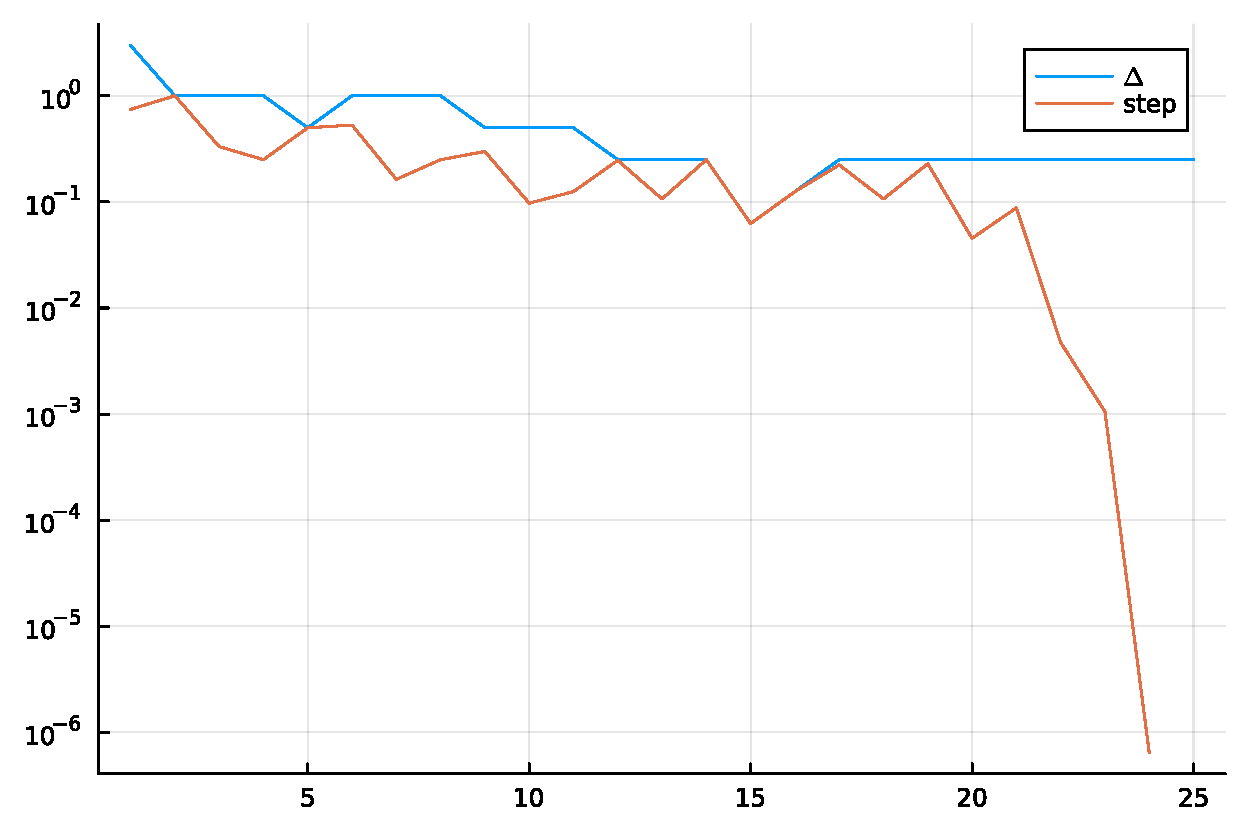
\includegraphics[width=0.8\textwidth]{fig/2023-04-19-banana-dhist.pdf}
\end{center}
\caption{Step size history for Rosenbrock banana example.}
\label{fig:banana-dhist}
\end{figure}

\begin{figure}
\begin{center}
  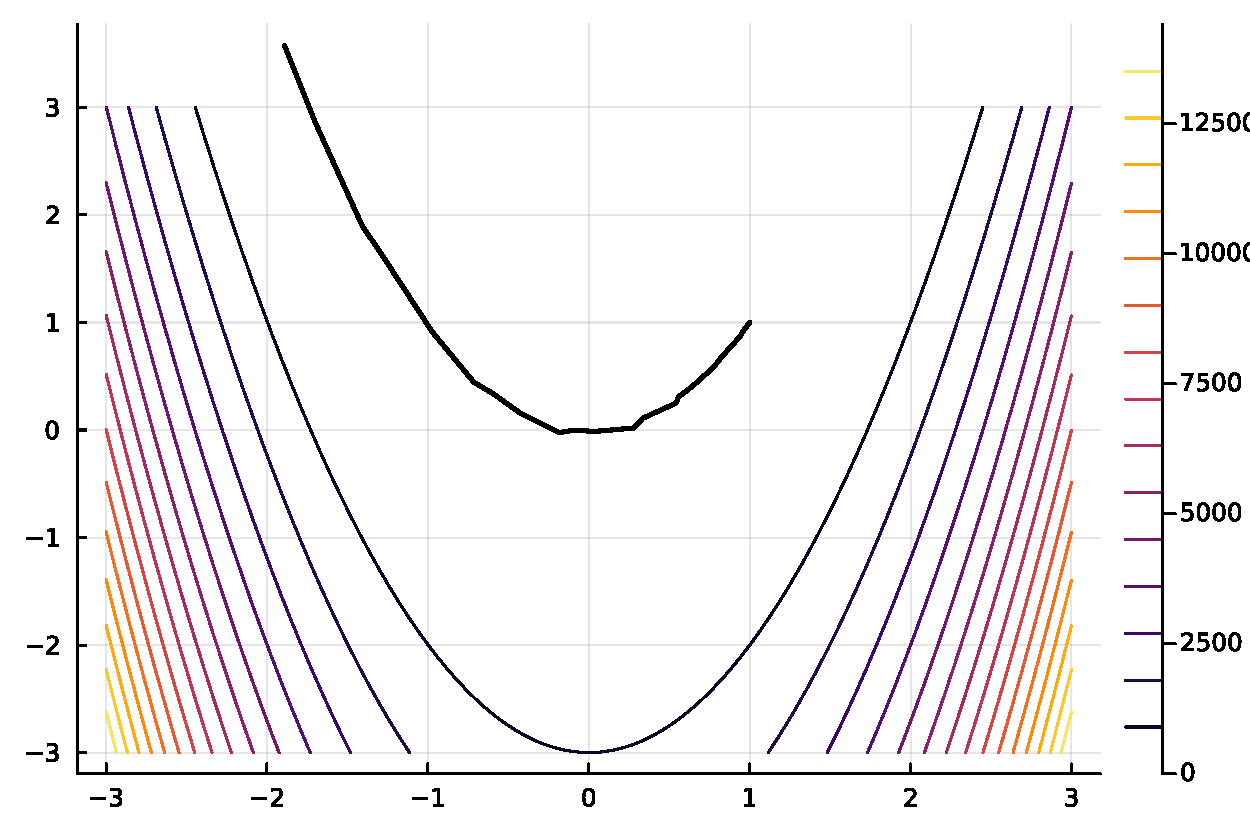
\includegraphics[width=0.8\textwidth]{fig/2023-04-19-banana-traj.pdf}
\end{center}
\caption{Solver trajectory for Rosenbrock banana example.}
\label{fig:banana-traj}
\end{figure}


\end{document}
